\documentclass[Protokollheft.tex]{subfiles}
\begin{document}
\chapter{HF-Zeitbereich 2: Leitungen und Ports}
%--------------- Start Vorbereitungsaufgaben ---------------

    Mit Hilfe der oben beschriebenen Ansätze sollen die Eigenschaften
    einer einfachen Koaxialleitung untersucht werden. Die Leitung wird
    Ihnen -- bereits diskretisiert -- in zwei Varianten in Form der Materialmatrizen
    $\Meps$ und $\Mmui$ vorgegeben. Im ersten Fall
    handelt es sich um eine homogene Leitung, im zweiten Fall enthält
    die Leitung einen dielektrischen Einsatz (siehe Abbildung~\ref{b1}).
    \begin{figure}[ht]
        \centering
        \begin{subfigure}{0.49\textwidth}
            \centering
            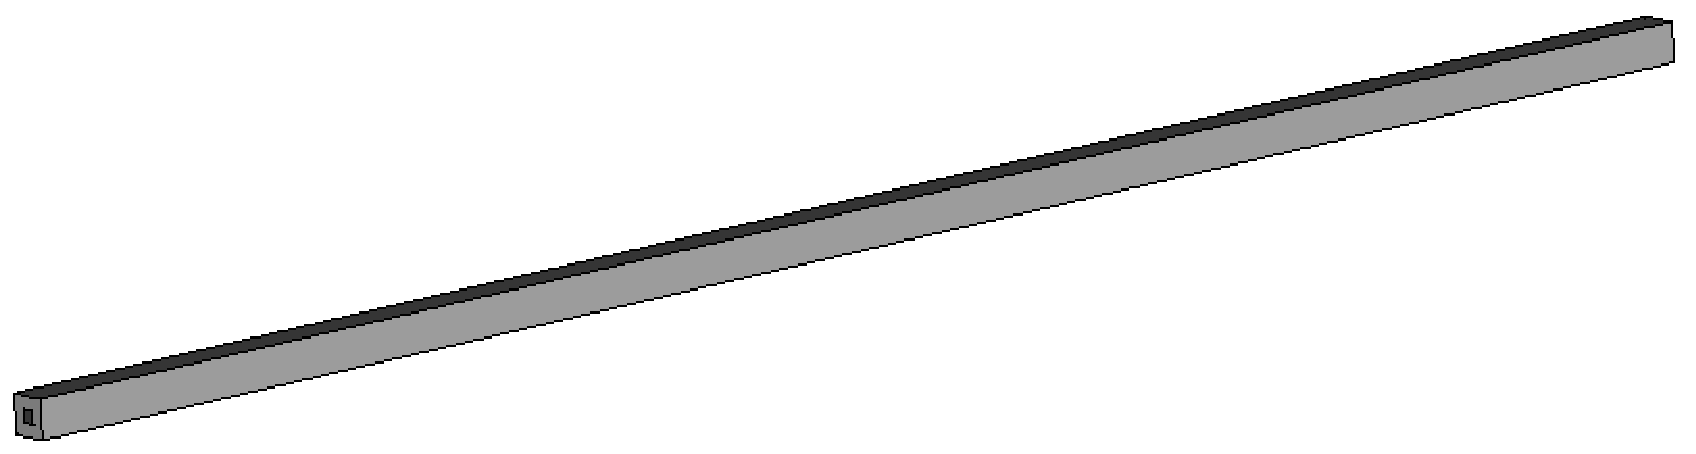
\includegraphics[width=8cm]{v7_homogen.pdf}
        \end{subfigure}
        \begin{subfigure}{0.49\textwidth}
            \centering
            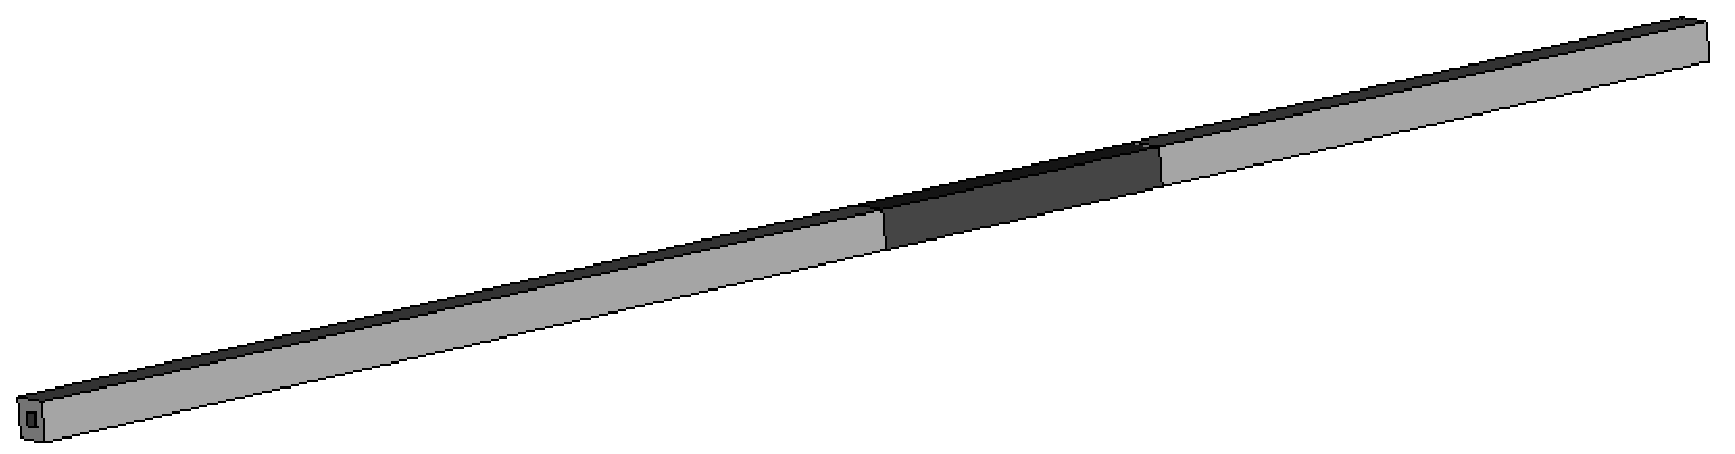
\includegraphics[width=8cm]{v7_inhomogen.pdf}
        \end{subfigure}
        \caption{Verlustfreie Koaxialleitung im Versuch. Es werden zwei Fälle vorgegeben: Eine homogene Koaxialleitung (links) und eine Koaxialleitung mit Einsatz (rechts).}\label{b1}
    \end{figure}
    Die Leitung selbst hat einen quadratischen Querschnitt mit
    ebenfalls quadratischem Innenleiter. Die Kantenlängen des
    Querschnitts betragen $3\,\text{cm}$, beziehungsweise $1\,\text{cm}$, die
    Leitungslänge ist $150\,\text{cm}$.
    Der Einsatz reicht von $75\,\text{cm}$ bis $100\,\text{cm}$.
    Alle Materialien sind als ideal angenommen. Der Innenleiter ist
    perfekt elektrisch leitend, die Dielektrika
    sind verlustfrei, im Fall der homogenen Leitung mit einem Wert von
    $\eps_\text{r}=1.3$, der Einsatz mit $\eps_\text{r}=10$. Die relative Permeabilität beträgt überall $\mur=1$. Der Außenleiter wird durch
    einen, bereits in die vorgegebenen Matrizen eingearbeiteten,
    elektrischen Rand modelliert. Das Grundmaterial wurde so gewählt,
    dass der Wellenwiderstand der Leitung $50\,\Omega$ beträgt.
    
    An den Stirnseiten (vgl. Abbildung~\ref{b3}) wurden, ebenfalls schon in den Matrizen
    enthalten, magnetische Randbedingungen angenommen. Die gesamte
    Struktur wurde mit einem homogenen Gitter mit $\Delta x = \Delta y
    = \Delta z = 1\,\text{cm}$ diskretisiert. Die Struktur enthält damit $4
    \times 4 \times 151$ Gitterpunkte.
    Das Gitter wurde für beide Leitungen identisch gewählt. Alle
    Vorüberlegungen sowie geschriebene Programmroutinen können direkt
    auf die Matrizen beider Strukturen angewendet werden. Als Anregung soll auf der vorderen Stirnseite ein Strom zwischen Innen- und Außenleiter eingeprägt werden. Die entsprechenden Kanten werden also im Laufe des Versuches mit einem Strom angeregt.
    \begin{figure}[h]
        \begin{center}
        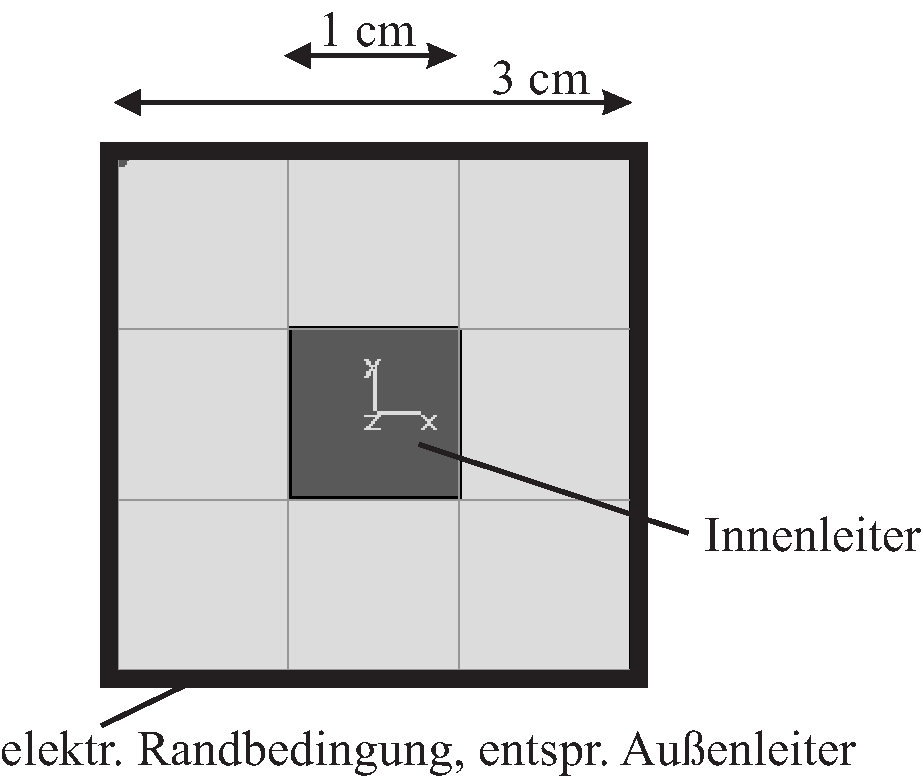
\includegraphics[width=8cm]{v7_mesh.pdf}
        \caption{Stirnseite der Koaxialleitung mit Diskretisierungsgitter.}\label{b3}
        \end{center}
    \end{figure}
    \newpage

\section{Vorbereitungsaufgaben}

% --> Aufgabe
\begin{framed}
	\noindent \textbf{1.} Weshalb ist es sinnvoll, für die Stirnseiten der Leitungen
magnetische Randbedingungen zu wählen?\label{exer:bound4frontOfLine}
\end{framed}

\emph{Fügen Sie hier Ihre Lösung ein}

% --> Aufgabe
\begin{framed}
	\noindent \textbf{2.} Das Gitter ist ein kanonisches kartesisches Gitter. Welchen
Indizes entsprechen diejenigen Kanten in der vorderen und der hinteren
Stirnfläche, die jeweils Innen- und Außenleiter miteinander
verbinden? Welchen Richtungssinn haben sie?\label{exer:idxConductorInterconnection}
\end{framed}

\emph{Fügen Sie hier Ihre Lösung ein}

% --> Aufgabe
\begin{framed}
	\noindent \textbf{3.} Nehmen Sie die erste Kante in $x$-Richtung, die Innen- und Außenleiter
miteinander verbindet und finden Sie die Indizes der
entsprechenden Kante, jeweils um einen $z$-Gitterschritt nach
hinten versetzt durch alle 151 Ebenen.\label{exer:idxEdge4allZ}
\end{framed}

\emph{Fügen Sie hier Ihre Lösung ein}

% --> Aufgabe
\begin{framed}
	\noindent \textbf{4.} Geben Sie die Funktion eines stückweise linearen
Trapezpulses in Abhängigkeit der Koordinaten der Knickpunkte an.\label{exer:calcPiecewiseTrapezoidal}
\end{framed}

\emph{Fügen Sie hier Ihre Lösung ein}

\begin{figure}[ht]
	\centering
    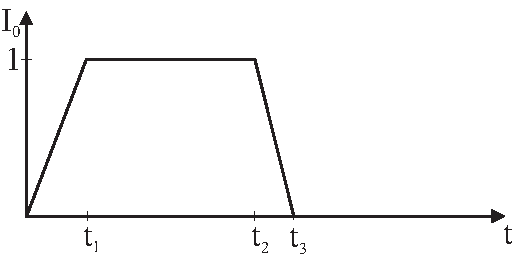
\includegraphics[scale=0.9]{v7_trapez.pdf}
    \caption{Trapezpuls}\label{tra}
\end{figure}

% --> Aufgabe
\begin{framed}
	\noindent \textbf{5.} Bestimmen Sie allgemein die Konstanten $\sigma$ und $t_0$
des Gaußpulses in Abhängigkeit der Maximalfrequenz $f_{\text{max}}$ 
und für $t_0$ zusätzlich auch in Abhängigkeit von $\sigma$. Bei
$f=f_{\text{max}}$ soll der Wert des Spektrums genau 1~\% des
Maximalwertes ($\sigma\sqrt{2\pi}$) betragen. Das zugehörige
Zeitsignal soll zum Zeitpunkt $t=0$ nur 0,1~\% seines
Maximalwertes betragen.\label{exer:calcGaussConst}
\end{framed}

\emph{Fügen Sie hier Ihre Lösung ein}

% --> Aufgabe
\begin{framed}
	\noindent \textbf{6.} Berechnen Sie die maximale Zeitschrittweite nach dem CFL-Kriterium.\label{exer:calcDeltaTmaxCFL}
\end{framed}

\emph{Fügen Sie hier Ihre Lösung ein}

\section{Aufgaben während der Praktikumssitzung}
Die vorliegende Beschreibung soll nur die grobe Vorgehensweise
während des Versuchs vorgeben. Sind die grundlegenden Dinge wie
Pulsgenerierung, modifizierter Leapfrog und visuelle Darstellung
implementiert, lassen sich verschiedene Pulsformen, verschiedene
Anregungen, Leitungsabschlüsse und die beiden Leitungen beliebig
miteinander kombinieren. Prinzipiell soll die Fortpflanzung eines
elektrischen Pulses über die vorgegebene Struktur visualisiert
werden. Dazu werden in jedem Zeitschritt die elektrischen Spannungen an hintereinander
liegenden Kanten über die z-Achse aufgetragen. Zum
selbstständigen Experimentieren soll hierbei durchaus ermutigt
werden. Der Hauptbestandteil der Implementierung in diesem Versuch soll in dem Skript \verb\versuch7.m\ erfolgen.

% --> Aufgabe
\begin{framed}
	\noindent \textbf{1.} Verwenden Sie die Leapfrog-Routine aus dem letzten Versuch. Nutzen Sie hierfür die bereits teilweise gegebene Methode \verb\leapfrog.m\, indem Sie den Eingabe-Parameter \verb\Rmat\ zunächst ignorieren.
Regen Sie eine beliebige Kante, die auf der vorderen Stirnfläche Innen-
und Außenleiter verbindet, an. Anregungssignal soll ein Trapezpuls
mit Anstiegs- und Abfallzeit $t_1=t_3-t_2=\SI{0,5}{ns}$ und einer
Haltezeit $t_2-t_1=\SI{0,7}{ns}$ sein. Es sollen zunächst 1000 Zeitschritte
berechnet werden. Speichern sie die elektrische Spannung der
von Ihnen ausgewählten Kante in jeder der 151 Ebenen ab. Plotten Sie damit
das elektrische Feld zwischen Innen- und Außenleiter in
Abhängigkeit von $z$ und verfolgen Sie den Verlauf über die Zeit
(als Film) mithilfe des {\texttt{drawnow}}-Befehls.\label{exer:visualizeTLine}
%
\end{framed}

\emph{Fügen Sie hier Ihre Lösung ein}

% --> Aufgabe
\begin{framed}
	\noindent \textbf{2.} Variieren Sie Ihre Leapfrog-Routine so, dass sie im
Folgenden auch konzentrierte Elemente berücksichtigen kann. Aus der Leitungstheorie 
ist bekannt, dass der Reflexionsfaktor $\Gamma$ bei einem Abschluss $Z_{\text{2}}$ am Ende der Leitung gerade 
\begin{align}
 \Gamma=\frac{Z_{\text{2}}-Z_{\text{w}}}{Z_{\text{2}}+Z_{\text{w}}},
\end{align}
mit dem Wellenwiderstand $Z_{\text{w}}$ beträgt. Für einen reflexionsfreien Abschluss soll die 
Leitung hier also mit ihrem Wellenwiderstand abgeschlossen werden,
indem einer der Kanten in der hinteren Stirnfläche ein Widerstand
von \SI{50}{\ohm} zugeordnet wird. Die Anzahl der Zeitschritte kann nach
eigenem Ermessen verringert werden. Der Durchlauf des Pulses durch
die Leitung soll auch in den weiteren Aufgabenteilen als Film
betrachtet werden.\label{exer:simIncludeLumped}\\
\textbf{Hinweis:} Benutzen Sie zum Berechnen der inversen Matrix 
in~(7.6) den Befehl \verb|nullInv|.
%
\end{framed}

\emph{Fügen Sie hier Ihre Lösung ein}

% --> Aufgabe
\begin{framed}
	\noindent \textbf{3.} Der Leitungsabschluss kann verbessert werden, indem der Gesamtwiderstand 
auf die acht Kanten verteilt wird. Vergleichen Sie das Reflexionsverhalten
mit dem in der vorherigen Teilaufgabe. Erklären Sie die Verbesserung!\label{exer:distributeTermination}
\end{framed}

\emph{Fügen Sie hier Ihre Lösung ein}

% --> Aufgabe
\begin{framed}
	\noindent \textbf{4.} Nun soll auch die Anregung symmetrisiert werden. Teilen Sie
den Anregungsstrom auf die acht Kanten der vorderen Stirnfläche
auf. Schließen Sie auch den vorderen Port reflexionsfrei ab.
Zeigen Sie die Verbesserung durch diese Maßnahme.\label{exer:symmetrizeExcitation}
\end{framed}

\emph{Fügen Sie hier Ihre Lösung ein}

% --> Aufgabe
\begin{framed}
	\noindent \textbf{5.} Verwenden Sie nun anstelle des Trapezpulses einen Gaußpuls
mit $f_{\text{max}}=\SI{1}{GHz}$. Was fällt bei der Ausbreitung im Vergleich
zum Trapezpuls auf?\label{exer:gaussExcitation}
\end{framed}

\emph{Fügen Sie hier Ihre Lösung ein}

% --> Aufgabe
\begin{framed}
	\noindent \textbf{6.} Verwenden Sie außer der homogenen Leitung nun auch die
inhomogene. Beachten Sie die Pulsform und
Ausbreitungsgeschwindigkeit innerhalb des dielektrischen
Einsatzes.\label{exer:inhomogenTLine}
\end{framed}

\emph{Fügen Sie hier Ihre Lösung ein}



\section{Fazit}
\emph{Fügen Sie hier Ihre Lösung ein}

\end{document}
